\documentclass{article}

% For figures
\usepackage{graphicx} % more modern
\usepackage{subfigure} 

% For citations
% \usepackage{natbib}

% For algorithms
\usepackage{algorithm}
\usepackage{algorithmic}

\usepackage{hyperref}

% Packages hyperref and algorithmic misbehave sometimes.  We can fix
% this with the following command.
\newcommand{\theHalgorithm}{\arabic{algorithm}}

% \usepackage{sty/icml2013} 
% Employ this version of the ``usepackage'' statement after the paper has
% been accepted, when creating the final version.  This will set the
% note in the first column to ``Proceedings of the...''
\usepackage[accepted]{sty/icml2013}


% The \icmltitle you define below is probably too long as a header.
% Therefore, a short form for the running title is supplied here:
\icmltitlerunning{Clustering and Topic Discovery in Gene Expression Data}

\begin{document} 

\twocolumn[
\icmltitle{Bayesian Clustering and Topic Discovery: \\ 
           Adventures with Gene Expression Data}

% It is OKAY to include author information, even for blind
% submissions: the style file will automatically remove it for you
% unless you've provided the [accepted] option to the icml2013
% package.
\icmlauthor{Karren Dai Yang, Skanda Koppula}{\{karren, skoppula\}@mit.edu}
\icmladdress{Massachusetts Institute of Technology,
            Cambridge, MA 02139 USA}

\icmlkeywords{topic models, bayesian clustering, gene expression, gene modules}

\vskip 0.3in
]

\section{Introduction}
\label{intro}
Tumors cell lines are composed of different sub-populations of cells which often exhibit shared patterns of gene expression. Biologists are interested in two key questions: given gene expressions values, (1) can we identify cell clusterings, and (2) can we identify clusters of biologically-related genes? Our goal with this project was to answer both these two questions using Bayesian methods.

In brief, we explored the use of three Bayesian clustering methods (a vanilla mixture, integrated topic-mixture, and non-parametric models) to address the first question, and two topic models (vanilla and a dynamic-topic LDA) to address the second. 

\subsection{Description of Data}
Using a contemporary gene sequencing machine, we obtained samples of single-cell RNA-sequencing data (scRNA-seq) taken from tumors in mice. Our data consisted of the expression values of 22,712 genes for each of 4645 cells. In total, the dataset amounted to 0.86 GB, presenting significant computational challenges when attempting posterior estimation. Apart from a few computational tricks (online inference, multi-core parallelization), for most methods, we pruned non-informative genes from the dataset, ranking based on the deviation in value across cells \footnote{We recognize that this can bias towards noisy genes. We favor this method because it is simple and easy to implement, and a practice used in literature \cite{pruning}}. We eschewed dimensionality reduction techniques such as PCA because of loss of its direct feature interpretability. The complete dataset, as well our preprocessed and pruned versions, are available at \cite{dataset}.

\subsection{Prior work}
Prior research has explored the use of various computational techniques to analyze gene expression data. Most commonly, Spearman and Pearson correlation metrics are frequently used infer sets of genes that cluster together \cite{profiling, nature}. Other techniques, including PCA followed by linear regression, has been used for expression-based cell clustering \cite{transcriptomics}. Yu et al. propose a unsupervised classifier ensemble as another approach to cell clustering \cite{consensus}. 

More Bayesian approaches have also been tried in prior work from the Pe'er lab. \cite{bayesge2} uses a Heirarchical Dirichlet Mixture Model to learn cell clusterings. \cite{bayesge1} builds on this to jointly learn optimal normalization pre-processing of the data. Bayesian networks have also been used in an attempt to learn gene dependencies from expression data \cite{bayesge3}.

\subsection{Structure of Report}
    We first discuss our experiments using Bayesian topic models to discover related sets of genes in a 'topic': LDA in Section~\ref{ldasec} and Dynamic Time Models in Section~\ref{dtmsec}. We discuss our experiments in clustering: Dirichlet Mixtures in Section~\ref{mmsec}, Integrated Topic-Clustering in Section~\ref{intsec}, and non-parametric models in Section~\ref{nonparametricsec}. Finally, we conclude our paper with our obversations from across all studies. 

\section{Latent Dirichlet Allocation} 
\label{ldasec}
\subsection{Model Description} 
In the generative process for LDA, the topic assigned to a word in a document is a drawn from the document's topic distribution. The identity of the word is drawn from topic's word distribution. Assuming the reader is familiar with LDA, we relegate further details and formalization of the model to \cite{LDA}.

In the context of analyzing gene expression data, we are interested in discovering 'topics' that comprise of a set of top-$N$ genes within the topic distribution that are biologically related. For example, together the genes may direct a specific chemical function in a cell. Biologists denote such sets of genes as 'gene modules' which can be cross-referenced with existing gene module databases.

\subsection{Implementation} 

\subsection{Experiments} 


\begin{figure}[h]
\vskip 0.2in
\begin{center}
\centerline{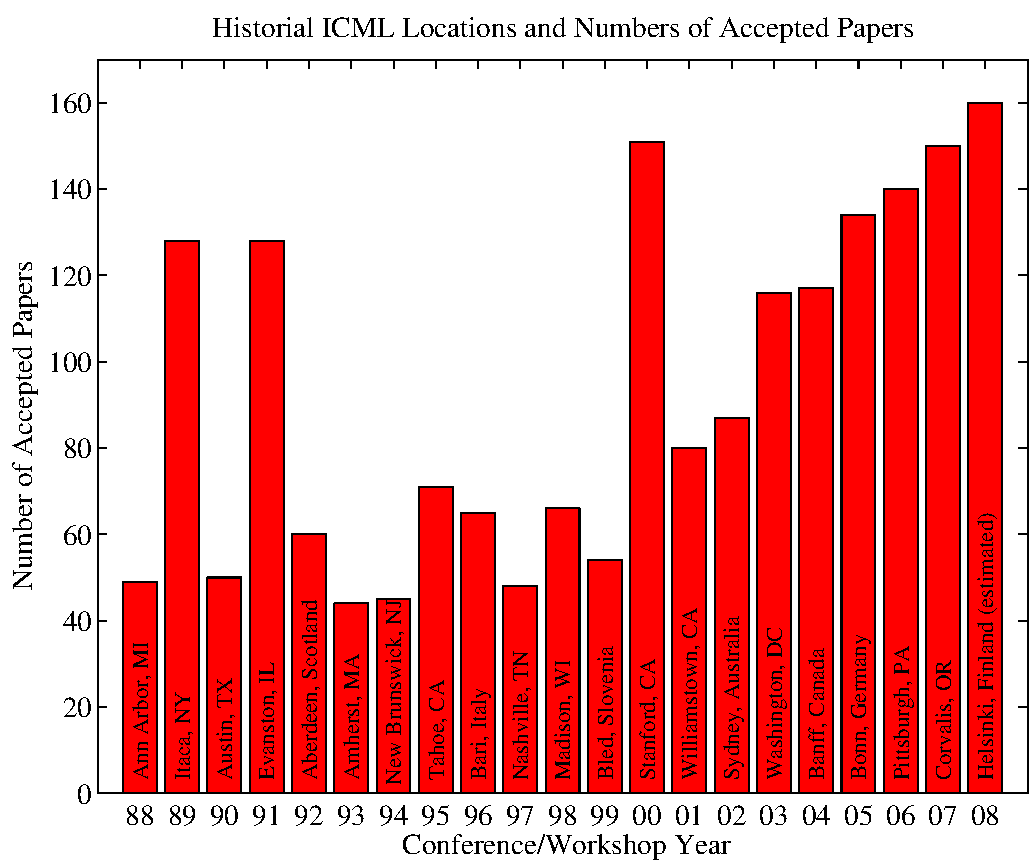
\includegraphics[width=\columnwidth]{figs/examplegraph}}
\caption{This is a demo figure.}
\label{alabel}
\end{center}
\vskip -0.2in
\end{figure} 





\section{Dirichlet Mixture Model} 
\label{mmsec}
\subsection{Model Description} 
    Algorithm~\ref{alg:example} describes the generative process for the mixture odel.

    \begin{algorithm}[tb]
       \caption{Mixture Model}
       \label{alg:example}
    \begin{algorithmic}
       \STATE {\bfseries Input:} data $x_i$, size $m$
       \REPEAT
       \STATE Initialize $noChange = true$.
       \FOR{$i=1$ {\bfseries to} $m-1$}
       \IF{$x_i > x_{i+1}$} 
       \STATE Swap $x_i$ and $x_{i+1}$
       \STATE $noChange = false$
       \ENDIF
       \ENDFOR
       \UNTIL{$noChange$ is $true$}
    \end{algorithmic}
    \end{algorithm}
\subsection{Implementation} 
\subsection{Experiments} 



\section{Dynamic Time Model} 
\label{dtmsec}
\subsection{Model Description} 
\subsection{Implementation} 
\subsection{Experiments} 




\section{Integrated Topic-Clustering Model} 
\label{intsec}
\subsection{Model Description} 
\subsection{Implementation} 
\subsection{Experiments} 



\section{Non-parametric Models: IBP and HDP} 
\label{nonparametricsec}
\subsection{Model Description} 
\subsection{Implementation} 
\subsection{Experiments} 


% In the unusual situation where you want a paper to appear in the
% references without citing it in the main text, use \nocite
% \nocite{langley00}

\bibliography{citations}
\bibliographystyle{sty/icml2013}


\section{Appendix} 
\subsection{Latent Dirichlet Allocation}

\end{document} 
